\paperchapter{December 2008}{7 December 2008}{C}{50}{GSET 2008}
\keytable{\kcell{1}{C} & \kcell{2}{D} & \kcell{3}{B} & \kcell{4}{D} & \kcell{5}{C} & \kcell{6}{B} & \kcell{7}{C} & \kcell{8}{A} & \kcell{9}{B} & \kcell{10}{A} \\
\kcell{11}{C} & \kcell{12}{C} & \kcell{13}{C} & \kcell{14}{C} & \kcell{15}{B} & \kcell{16}{B} & \kcell{17}{D} & \kcell{18}{A} & \kcell{19}{A} & \kcell{20}{D} \\
\kcell{21}{B} & \kcell{22}{D} & \kcell{23}{A} & \kcell{24}{C} & \kcell{25}{C} & \kcell{26}{C} & \kcell{27}{B} & \kcell{28}{D} & \kcell{29}{C} & \kcell{30}{C} \\
\kcell{31}{A} & \kcell{32}{C} & \kcell{33}{D} & \kcell{34}{D} & \kcell{35}{B} & \kcell{36}{B} & \kcell{37}{A} & \kcell{38}{C} & \kcell{39}{B} & \kcell{40}{C} \\
\kcell{41}{D} & \kcell{42}{A} & \kcell{43}{C} & \kcell{44}{C} & \kcell{45}{D} & \kcell{46}{C} & \kcell{47}{B} & \kcell{48}{C} & \kcell{49}{C} & \kcell{50}{B}}
\begin{question}{1}
{If TEAM is coded as VGCO, then LIFE will be coded as:\par}
\optsfour{NJGE}{NKHF}{NKHG}{NLIH}
\answer{C}{NKHG}
\begin{explain}
Each letter moves \textbf{two places forward}: T$\rightarrow$V, E$\rightarrow$G, A$\rightarrow$C, M$\rightarrow$O.
LIFE $\rightarrow$ L$+2=$N, I$+2=$K, F$+2=$H, E$+2=$G, giving \textbf{NKHG}.
\end{explain}
\end{question}

\begin{question}{2}
{Which of the alternatives will fit in ?\par}
\qfigure{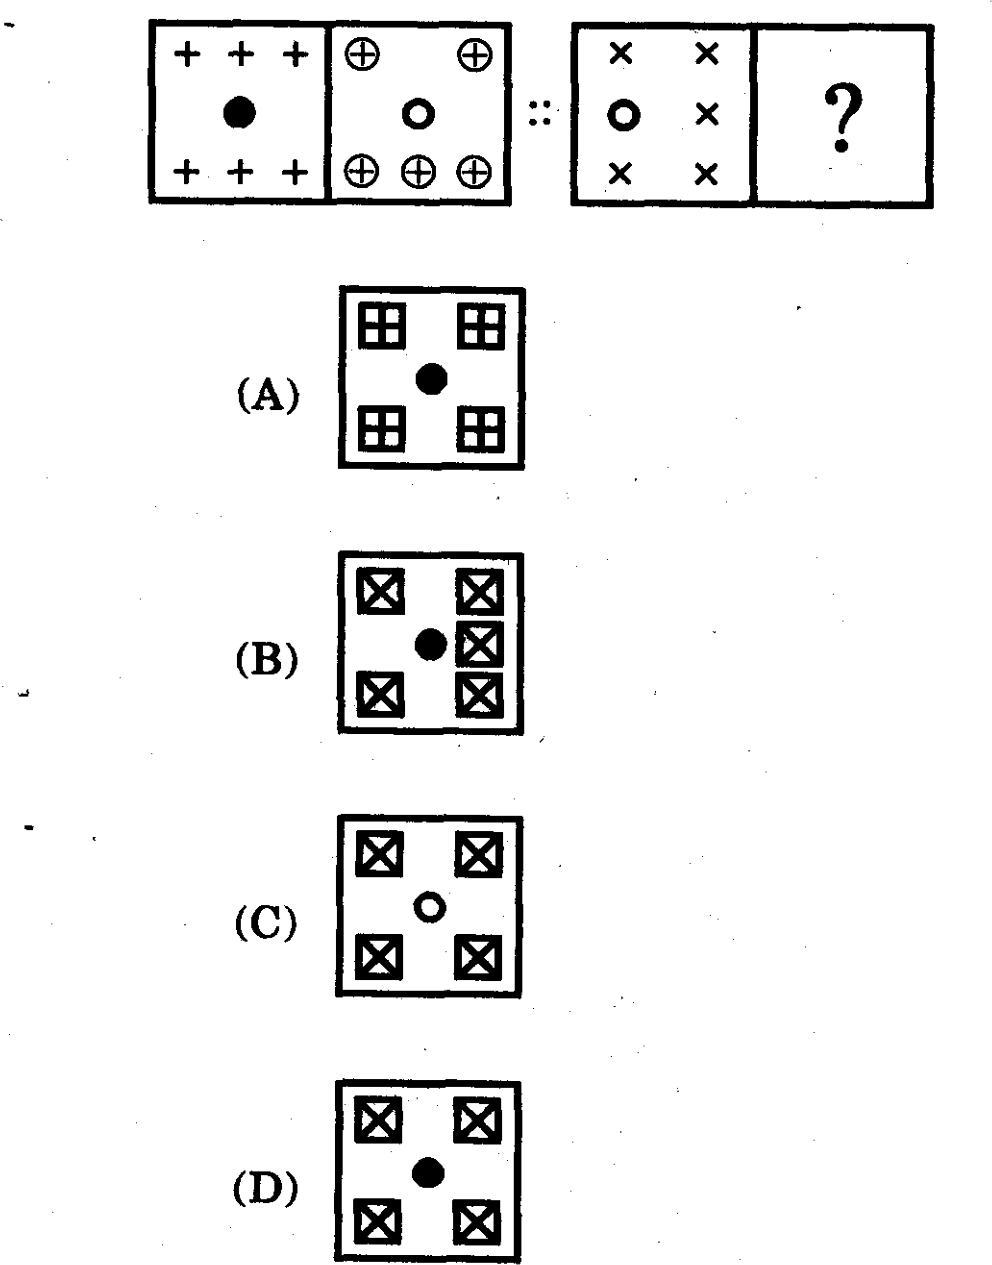
\includegraphics[height=6.2cm]{fig/dec08_q2.png}}
\optsfour{Figure (A)}{Figure (B)}{Figure (C)}{Figure (D)}
\answer{D}{Figure (D)}
\begin{explain}
From the first figure to the second, three things happen. Each symbol is \textbf{enclosed} ($+\rightarrow\oplus$), the number of symbols \textbf{falls by one} ($6\rightarrow5$), and the central dot \textbf{changes shade} (filled $\rightarrow$ hollow).
Apply the same to the third figure: $\times\rightarrow\boxtimes$, $5\rightarrow4$ symbols, and the hollow dot becomes \textbf{filled}. Figure \textbf{(D)} fits.
\why{(A) uses boxed plus signs; (B) has five symbols; (C) keeps the dot hollow.}
\end{explain}
\end{question}

\begin{question}{3}
{How many 7's are there in the following number series which are not followed by 3 but are preceded by 8? 898762263269732872778737794\par}
\optsfour{10}{2}{3}{0}
\answer{B}{2}
\begin{explain}
Look for the pattern ``8 7 x'' where x $\neq 3$:
\begin{center}\ttfamily 8 9 8 \textbf{7} 6 2 2 6 3 2 6 9 7 3 2 8 \textbf{7} 2 7 7 8 7 3 7 7 9 4\end{center}
``8 7 6'' (position 3--5) and ``8 7 2'' qualify, while ``8 7 3'' is excluded. Count $=\mathbf{2}$.
\end{explain}
\end{question}

\begin{question}{4}
{Nitin is counting the numbers in descending order from 32. Shashank is counting the numbers in ascending order from 1 and he pronounces only the odd numbers. If they are counting with the same speed which same number will they pronounce together?\par}
\optstwo{21}{22}{19}{None of the above}
\answer{D}{None of the above}
\begin{explain}
Nitin says 32, 31, 30, \ldots; Shashank says 1, 3, 5, \ldots. At the $n$-th count Nitin says $33-n$ and Shashank says $2n-1$.
$33-n=2n-1\Rightarrow n=34/3$, which is not a whole number, so they \textbf{never say the same number together}: none of the above.
\end{explain}
\end{question}

\begin{question}{5}
{In the following, English letters are used for various symbols: 'B' for addition, 'G' for subtraction, 'E' for multiplication, 'C' for division, 'D' for equal, 'A' for > and 'F' for <. Which of the following is correct?\par}
\optstwo{18C3D6B8C4G12}{18A13B16E8G4E12}{18C3G6B8B4D12}{18A3E6B8G4B12}
\answer{C}{18C3G6B8B4D12}
\begin{explain}
Decode (C): $18\div3-6+8+4=12$, i.e.\ $6-6+8+4=12$ \checkmark.
Check the others: (A) $18\div3=6$ but the right side $8\div4-12$ is not 6; (B) $18>13+128-48$ is false; (D) $18>18+8-4+12=34$ is false.
\end{explain}
\end{question}

\begin{question}{6}
{Numbers are placed in the following figure on the basis of some rules. One place is vacant which is indicated as (?). Find the correct alternative for vacant place.\par}
\qfigure{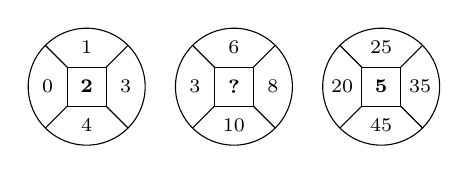
\begin{tikzpicture}[scale=0.55,font=\scriptsize]
\foreach \cx/\t/\l/\r/\b/\c in {0/1/0/3/4/2, 3.4/6/3/8/10/?, 6.8/25/20/35/45/5}{
 \draw (\cx,0) circle(1.35); \draw (\cx-0.45,-0.45) rectangle (\cx+0.45,0.45);
 \draw (\cx-0.45,0.45)--(\cx-0.95,0.95); \draw (\cx+0.45,0.45)--(\cx+0.95,0.95);
 \draw (\cx-0.45,-0.45)--(\cx-0.95,-0.95); \draw (\cx+0.45,-0.45)--(\cx+0.95,-0.95);
 \node at (\cx,0.9){\t}; \node at (\cx-0.9,0){\l}; \node at (\cx+0.9,0){\r}; \node at (\cx,-0.9){\b}; \node at (\cx,0){\textbf{\c}};}
\end{tikzpicture}}
\optsfour{2}{3}{7}{9}
\answer{B}{3}
\begin{explain}
The centre number is the \textbf{cube root of the sum} of the four outer numbers:
\[0+3+1+4=8=2^3,\qquad 20+35+25+45=125=5^3\]
\[3+8+6+10=27=3^3\ \Rightarrow\ ?=\mathbf{3}\]
\end{explain}
\end{question}

\begin{question}{7}
{In a survey of 60 people, it was found that 25 read Newsweek magazine; 26 read Time; 26 read Fortune; 9 read both Newsweek and Fortune; 11 read both Newsweek and Time; 8 read both Time and Fortune and 3 read all magazines. Then number of people who read only Newsweek; Time and Fortune respectively are\par}
\optsfour{7, 10 and 12}{8, 11 and 12}{8, 10 and 12}{8, 10 and 13}
\answer{C}{8, 10 and 12}
\begin{explain}
Let N, T, F be the readers. Only Newsweek $=25-(9+11-3)=25-17=\mathbf{8}$; only Time $=26-(11+8-3)=26-16=\mathbf{10}$; only Fortune $=26-(9+8-3)=26-14=\mathbf{12}$.
\begin{center}
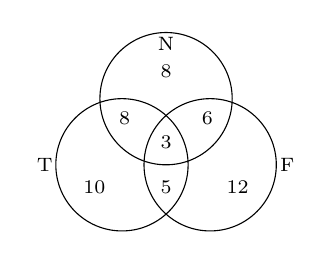
\begin{tikzpicture}[scale=0.7,font=\scriptsize]
\draw (0,0.6) circle(1.2) node[above=14pt]{N}; \draw (-0.8,-0.6) circle(1.2); \draw (0.8,-0.6) circle(1.2);
\node at (0,1.1){8}; \node at (-1.3,-1.0){10}; \node at (1.3,-1.0){12};
\node at (-0.75,0.25){8}; \node at (0.75,0.25){6}; \node at (0,-1.0){5}; \node at (0,-0.2){3};
\node at (-2.2,-0.6){T}; \node at (2.2,-0.6){F};
\end{tikzpicture}
\end{center}
(N$\cap$T only $=11-3=8$, N$\cap$F only $=9-3=6$, T$\cap$F only $=8-3=5$.)
\end{explain}
\end{question}

\begin{question}{8}
{Which of the following best represents the relationship among tennis fans, cricket players and students?\par}
\optsfour{\tikz[baseline=-0.5ex,scale=0.28]{\draw (0,0.45) circle(1); \draw (-0.55,-0.45) circle(1); \draw (0.55,-0.45) circle(1);}}{\tikz[baseline=-0.5ex,scale=0.28]{\draw (0,0) circle(1.3); \draw (0,0.35) circle(0.5); \draw (0,-0.35) circle(0.5);}}{\tikz[baseline=-0.5ex,scale=0.28]{\draw (0,0) circle(0.8); \draw (1.1,0) circle(0.8); \draw (2.2,0) circle(0.8);}}{\tikz[baseline=-0.5ex,scale=0.28]{\draw (0,0) circle(1.2); \draw (0,0) circle(0.9); \draw (0.9,0) circle(0.8);}}
\answer{A}{\tikz[baseline=-0.5ex,scale=0.28]{\draw (0,0.45) circle(1); \draw (-0.55,-0.45) circle(1); \draw (0.55,-0.45) circle(1);}}
\begin{explain}
Tennis fans, cricket players and students can all overlap (a student may play cricket and follow tennis), and none contains another. So we need \textbf{three mutually intersecting circles}, as in diagram (A).
\end{explain}
\end{question}

\begin{question}{9}
{When a parachutist jumps off a plane and the parachute opens, the total force on the man is:\par}
\optstwo{greater than his weight}{less than his weight}{equal to his weight}{zero}
\answer{B}{less than his weight}
\begin{explain}
When the parachute opens, air resistance acts upward. The \textbf{net (total) force} on the man is his weight minus the drag, which is \textbf{less than his weight}. It falls to zero only when he reaches terminal velocity.
\end{explain}
\end{question}

\begin{question}{10}
{Consider the sequence : 0, 1, 1, 2, 3, 5, 8, 13, 21, 34, \ldots{} The next four members of sequence are:\par}
\optstwo{55, 89, 144 and 233}{45, 79, 134 and 223}{65, 99, 154 and 243}{54, 89, 144 and 232}
\answer{A}{55, 89, 144 and 233}
\begin{explain}
This is the \textbf{Fibonacci sequence}: each term is the sum of the previous two. $21+34=55$, $34+55=89$, $55+89=144$, $89+144=233$.
\end{explain}
\end{question}

\begin{question}{11}
{Read the following graph and decide which of the following statement is \emph{false}:\par}
\qfigure{\begin{tikzpicture}
\begin{axis}[ybar,width=8cm,height=4.4cm,bar width=16pt,ymin=0,ymax=400,
  symbolic x coords={1995-96,1996-97,1997-98,1998-99,1999-2000},xtick=data,
  nodes near coords,every node near coord/.append style={font=\tiny},tick label style={font=\scriptsize},
  ylabel={\scriptsize Students in Class I},axis x line*=bottom,axis y line*=left]
\addplot[pattern=north east lines,draw=ink] coordinates {(1995-96,150) (1996-97,200) (1997-98,250) (1998-99,300) (1999-2000,350)};
\end{axis}
\end{tikzpicture}}
\optsone{Number of students in each academic year is divisible by 25}{Number of students in 1999-2000 is more than twice the number in 1995-96}{Number of students in 1995-96: Number of students in 1996-97 is equal to Number of students in 1996-97: No. of students in 1997-98}{The total growth in number of students is not less than 200}
\answer{C}{Number of students in 1995-96: Number of students in 1996-97 is equal to Number of students in 1996-97: No. of students in 1997-98}
\begin{explain}
Values: 150, 200, 250, 300, 350.
(A) all are divisible by 25, true. (B) $350>2\times150=300$, true. (D) total growth $=350-150=200$, which is not less than 200, true.
(C) $150:200=0.75$ but $200:250=0.8$, so the ratios are \textbf{not equal}. Statement (C) is \textbf{false}.
\end{explain}
\end{question}

\begin{question}{12}
{Following the constant growth described in the previous diagram, which year first time there will be more than 1111 students in Class I ?\par}
\optsfour{2010}{2013}{2016}{2020}
\answer{C}{2016}
\begin{explain}
Growth is constant at $+50$ students per year: $350+50n>1111\Rightarrow n>15.22\Rightarrow n=16$.
Sixteen years after 1999--2000 is 2015--16, i.e.\ \textbf{2016}.
\end{explain}
\end{question}

\begin{question}{13}
{A tyre manufacturing company kept a record of the distance covered before a tyre to be replaced. The following table shows the results of 1000 cases:
\begin{center}\small
\begin{tabular}{lc}\toprule Distance (km) & Tyres replaced\\\midrule Less than 400 & 210\\ 400--900 & 325\\ 900--1400 & 385\\ More than 1400 & 80\\\bottomrule\end{tabular}
\end{center}
If you buy a tyre of this company, what is the probability that it will need to be replaced before it has covered 400 km?\par}
\optsfour{0.4}{0.3}{0.21}{0.14}
\answer{C}{0.21}
\begin{explain}
Empirical probability $=\dfrac{210}{1000}=\mathbf{0.21}$.
\end{explain}
\end{question}

\begin{question}{14}
{As a researcher you find that, the correlation between intensity of punishment and students' achievement is -.86. This means that:\par}
\optsone{higher the intensity of punishment greater would be the achievement}{intensity of punishment has no relation with achievement}{increase in the intensity of punishment will decrease achievement of students}{increase in the intensity of punishment may or may not decrease the achievement of students}
\answer{C}{increase in the intensity of punishment will decrease achievement of students}
\begin{explain}
A correlation of $-0.86$ is a \textbf{high negative} correlation: as the intensity of punishment increases, achievement tends to \textbf{decrease}.
\tip{Correlation shows association, not proof of causation, but in exam language this is read as ``more punishment, lower achievement''.}
\end{explain}
\end{question}

\begin{question}{15}
{In an experimental study you want to study the effectiveness of method of teaching A and B. Each group has 50 randomly selected students. Appropriate technique of data analysis will be :\par}
\optstwo{chi-square test}{t-test}{F-test}{multiple regression}
\answer{B}{t-test}
\begin{explain}
Comparing the means of \textbf{two independent groups} (method A vs method B), each of 50 students, calls for the \textbf{t-test}.
\why{Chi-square is for frequencies; the F-test (ANOVA) is for three or more groups; regression is for prediction.}
\end{explain}
\end{question}

\begin{question}{16}
{Which of the following is used to connect two LAN using same LAN protocols over a wide area ?\par}
\optstwo{Router}{Bridges}{Gateways}{None of the above}
\answer{B}{Bridges}
\begin{explain}
Per the key, \textbf{bridges} connect two LANs that use the same protocol. (Bridges work at the data-link layer; routers connect different networks.)
\end{explain}
\end{question}

\begin{question}{17}
{Which of the following are switching techniques ?\par}
\optstwo{Circuit switching}{Message switching}{Packet switching}{Each of the above three techniques}
\answer{D}{Each of the above three techniques}
\begin{explain}
Circuit switching (telephone), message switching (store-and-forward) and packet switching (Internet) are all switching techniques: \textbf{each of the three}.
\end{explain}
\end{question}

\begin{question}{18}
{Protocol is used to communicate between:\par}
\optstwo{similar module}{dissimilar module}{both (A) and (B)}{none of the above}
\answer{A}{similar module}
\begin{explain}
A \textbf{protocol} is a set of rules for communication between \textbf{similar (peer) modules}, i.e.\ the same layer in two systems.
\end{explain}
\end{question}

\begin{question}{19}
{Data transfer rate for LAN is normally:\par}
\optstwo{1-100 Mbps}{1-2 Mbps}{1-10 Mbps}{None of the above}
\answer{A}{1-100 Mbps}
\begin{explain}
Typical LAN data rates are \textbf{1--100 Mbps} (Ethernet 10/100 Mbps in that period).
\end{explain}
\end{question}

\begin{question}{20}
{Which of the following are WAN devices ?\par}
\optstwo{Bridges}{Routers}{Gateways}{Each of the above three devices}
\answer{D}{Each of the above three devices}
\begin{explain}
Bridges, routers and gateways are all used in wide-area networking: \textbf{each of the three devices}.
\end{explain}
\end{question}

\begin{question}{21}
{Mushrooms form a promising source of:\par}
\optstwo{carbohydrate}{protein}{minerals}{carbohydrate plus lipid}
\answer{B}{protein}
\begin{explain}
Mushrooms are valued as a promising source of \textbf{protein} (with vitamins and minerals), especially for vegetarians.
\end{explain}
\end{question}

\begin{question}{22}
{Nuclear energy can be obtained from:\par}
\optsone{fission of radioactive material}{synthetic reactions of radioactive material}{fusion of radioactive material}{both fission and fusion of radioactive material}
\answer{D}{both fission and fusion of radioactive material}
\begin{explain}
Nuclear energy comes from both \textbf{fission} (splitting heavy nuclei such as U-235) and \textbf{fusion} (joining light nuclei, as in the Sun).
\end{explain}
\end{question}

\begin{question}{23}
{Petroplants are the sources of:\par}
\optstwo{liquid hydrocarbon}{liquid nitrogen}{liquid fuels}{alcohols}
\answer{A}{liquid hydrocarbon}
\begin{explain}
\textbf{Petroplants} (e.g.\ \emph{Euphorbia}, \emph{Jatropha}) yield latex rich in \textbf{liquid hydrocarbons} that can substitute for petroleum.
\end{explain}
\end{question}

\begin{question}{24}
{Occupational diseases result from:\par}
\optstwo{malnutrition}{overworking}{toxic chemical residues}{unadequate basic amenities}
\answer{C}{toxic chemical residues}
\begin{explain}
Occupational diseases (silicosis, asbestosis, lead poisoning) result from exposure to \textbf{toxic chemicals, dusts and residues} at the workplace.
\end{explain}
\end{question}

\begin{question}{25}
{Which one among the following is a non-commercial sources of energy ?\par}
\optstwo{Coal}{Oil}{Agricultural waste}{Electricity}
\answer{C}{Agricultural waste}
\begin{explain}
\textbf{Agricultural waste} (together with firewood and cow dung) is a \textbf{non-commercial} energy source: it is not usually bought and sold. Coal, oil and electricity are commercial.
\end{explain}
\end{question}

\begin{question}{26}
{The research in education has not given due importance to:\par}
\optstwo{adolescent student's problems}{adolescent learning styles}{adult student's learning styles}{children's learning styles}
\answer{C}{adult student's learning styles}
\begin{explain}
Educational research has concentrated on children and adolescents and has given relatively little importance to \textbf{adult students' learning styles} (andragogy).
\end{explain}
\end{question}

\begin{question}{27}
{Linking Career Advancement Scheme with research publications:\par}
\optsone{enhances quality of research due to increase in quantity}{deteriorates quality of research due to increase in quantity}{enhances quality of research as fund of knowledge is greater}{does not influence quality of research}
\answer{B}{deteriorates quality of research due to increase in quantity}
\begin{explain}
Per the key, linking career advancement to the number of publications \textbf{deteriorates quality}: it encourages quantity over quality (``publish or perish'', predatory journals).
\end{explain}
\end{question}

\begin{question}{28}
{Which of the following IGNOU does not prescribe ?\par}
\optsone{Flexibility to eligibility for enrolment}{Relaxation of age of entry}{Flexibility to methods of evaluation}{Strict combination of courses of study}
\answer{D}{Strict combination of courses of study}
\begin{explain}
IGNOU offers flexibility in eligibility, age of entry, pace and evaluation. It does \emph{not} prescribe a \textbf{strict combination of courses}; learners may choose.
\end{explain}
\end{question}

\begin{question}{29}
{Spiritual value never cherishes:\par}
\optstwo{non-violence}{respect for all religions}{untouchability}{truth}
\answer{C}{untouchability}
\begin{explain}
Spiritual values include non-violence, truth and respect for all religions. \textbf{Untouchability} contradicts them (it is also abolished by Article 17).
\end{explain}
\end{question}

\begin{question}{30}
{The POA of NPE, 1992 does not envisage:\par}
\optsone{making education a mass movement}{special emphasis on education of girls}{making English as compulsory language for all}{establishment of pace-setting institutions}
\answer{C}{making English as compulsory language for all}
\begin{explain}
The Programme of Action (1992) of NPE 1986 aimed at a mass movement for education, girls' education and pace-setting institutions (Navodaya Vidyalayas). It did not make \textbf{English compulsory for all}.
\end{explain}
\end{question}

\begin{question}{31}
{Which is not the aim of education ?\par}
\optsone{Completing the syllabus in stipulated time}{Inculcating cognitive competence through subject teaching}{Developing citizenship in the students}{Equipping students with life skills}
\answer{A}{Completing the syllabus in stipulated time}
\begin{explain}
\textbf{Completing the syllabus in stipulated time} is an administrative target, not an aim of education.
\end{explain}
\end{question}

\begin{question}{32}
{What will you do to update your competence of teaching?\par}
\optsone{Read books on methods of teaching}{Visit different websites on teaching techniques}{Experimenting with a variety of classroom activities}{Seek guidance from senior teachers}
\answer{C}{Experimenting with a variety of classroom activities}
\begin{explain}
The best way to update teaching competence is to \textbf{experiment with a variety of classroom activities}, i.e.\ reflective practice and learning by doing.
\end{explain}
\end{question}

\begin{question}{33}
{If a learner can use an abstraction-a rule, a principle or an idea in particular and concrete situations, then he has reached the level of educational objective:\par}
\optsfour{comprehension}{analysis}{synthesis}{application}
\answer{D}{application}
\begin{explain}
Using an abstraction (rule, principle) in particular, concrete situations is \textbf{application} in Bloom's taxonomy.
\end{explain}
\end{question}

\begin{question}{34}
{How is the working model valued ?\par}
\optsone{By recognition of external features}{By seeing the internal structure}{By seeing both external and internal structures}{By following actions and processes as they develop}
\answer{D}{By following actions and processes as they develop}
\begin{explain}
A working model is valued for \textbf{showing actions and processes as they develop}, i.e.\ how the thing actually works.
\end{explain}
\end{question}

\begin{question}{35}
{Adolescents' problems may be handled by those teachers who have skills of:\par}
\optsfour{Managers}{Counsellors}{Psychiatrists}{Therapists}
\answer{B}{Counsellors}
\begin{explain}
Adolescents' problems are best handled by teachers with \textbf{counselling} skills.
\end{explain}
\end{question}

\begin{question}{36}
{In research operational definition of a variable means:\par}
\optsone{considering different definitions and giving one's own as taken in the present study}{stipulating tasks by which variables can be observed and measured}{explaining operationality to make concept clear}{stipulating concept in all its constituents}
\answer{B}{stipulating tasks by which variables can be observed and measured}
\begin{explain}
An \textbf{operational definition} states the operations or tasks by which a variable is \textbf{observed and measured} (e.g.\ ``achievement $=$ score on test X'').
\end{explain}
\end{question}

\begin{question}{37}
{In an experimental research, it is essential that researcher :\par}
\optsone{directly controls and manipulates variables}{must take things as they are in an experiment}{must manipulate the variable but need not control}{must control the variable but need not manipulate}
\answer{A}{directly controls and manipulates variables}
\begin{explain}
In experimental research the researcher \textbf{directly manipulates} the independent variable and \textbf{controls} extraneous variables.
\end{explain}
\end{question}

\begin{question}{38}
{The research aims at understanding reality, discovering new knowledge and inventions for development in the society and research ethics certainly can restrain researchers. Considering all aspects it is amicably decided that researchers :\par}
\optsone{will have complete freedom for research}{will not conduct studies involving risks to human beings}{will follow some code of research ethics}{will decide research ethics themselves}
\answer{C}{will follow some code of research ethics}
\begin{explain}
Research must balance freedom and responsibility, so researchers \textbf{follow a code of research ethics} (informed consent, confidentiality, avoidance of harm).
\end{explain}
\end{question}

\begin{question}{39}
{The law of probability is applied in:\par}
\optstwo{purposive sampling}{random sampling}{quota sampling}{convenient sampling}
\answer{B}{random sampling}
\begin{explain}
The law of probability applies to \textbf{random sampling}, where each unit has a known, equal chance of selection.
\end{explain}
\end{question}

\begin{question}{40}
{If a researcher wants to study the performance of university teachers by students which tool will be most appropriate ?\par}
\optstwo{Questionnaire}{Interview}{Rating scale}{Observation schedule}
\answer{C}{Rating scale}
\begin{explain}
To obtain students' evaluation of teacher performance on various dimensions, a \textbf{rating scale} is the most appropriate tool.
\end{explain}
\end{question}

\begin{context}
\textbf{Direction (Q.~Nos.~41 to 45):} Read the following text and answer the questions that follow.\par\smallskip
Human decision-making is being influenced profoundly by modern mathematics, and several particular mathematical subjects have been created primarily to assist in arriving at good decisions. Many aspects involved in arriving at a decision are, of course, nonquantitative in nature. These may relate to history, past experience, instinct, judgement, morality, and so forth. As a consequence, one often refers to decision-making as an art. On the other hand, many ingredients in contemporary decision-making are mathematical in nature, and one can also view this activity as a science.

A decision maker will begin by listing the options over which he or she has some control and the likely outcomes resulting from these choices. The person may attempt to identify all relevant variables and the relationships among them and may associate quantitative measures when possible. Moreover, the decision maker must clarify his or her own values, identify desired goals, and spell out explicitly any limiting resources or social constraints. One then seeks the best possible result obtainable. The situation is typically confounded by a variety of different uncertainties involving data and forecasting that typically cannot be completely resolved in advance. The effect that other decision makers may have on the outcome, and the best responses to their moves, should be predetermined. Various ethical concerns such as fairness may well need consideration, and ways to ascertain group opinions may be necessary. Finally, decision makers must study the social and political context in which the decision will be implemented.
\end{context}
\begin{question}{41}
{What is the central idea of this paragraph ?\par}
\optsone{Decision-making is a mathematical activity}{Decision-making is a complex intellectual activity}{Decision-making is almost impossible}{Decision-making is also emotional and social in nature}
\answer{D}{Decision-making is also emotional and social in nature}
\begin{explain}
The passage stresses that besides mathematics, decision-making involves non-quantitative aspects (history, instinct, judgement, morality), group opinion and the social--political context. Per the key, the central idea is that it is \textbf{also emotional and social in nature}.
\end{explain}
\end{question}

\begin{question}{42}
{What is the major source of puzzlement in decision-making ?\par}
\optsone{An exact prediction of the results of the decision}{Socio-political context}{Ignorance of Mathematics}{Lack of adequate practice}
\answer{A}{An exact prediction of the results of the decision}
\begin{explain}
The situation ``is typically confounded by a variety of different uncertainties involving data and forecasting that typically cannot be completely resolved in advance'', i.e.\ the difficulty of \textbf{exactly predicting the results}.
\end{explain}
\end{question}

\begin{question}{43}
{Which step is not inevitable in the process of decision-making ?\par}
\optsone{Recognizing the factors affecting the process}{Thinking of the end product one would wish to achieve}{Using quantitative measures}{Forecasting outcomes in advance}
\answer{C}{Using quantitative measures}
\begin{explain}
The decision maker ``may associate quantitative measures \textbf{when possible}'', so using quantitative measures is \textbf{not inevitable}. The other steps are described as necessary.
\end{explain}
\end{question}

\begin{question}{44}
{Decision-making is an art, because:\par}
\optsone{it involves a lot of variables}{it depends upon a person's multiple abilities}{it entails some personal perspectives}{it does not ensure the best outcome}
\answer{C}{it entails some personal perspectives}
\begin{explain}
Decision-making is called an art because many aspects are non-quantitative: history, experience, instinct, judgement, morality, i.e.\ it \textbf{entails personal perspectives}.
\end{explain}
\end{question}

\begin{question}{45}
{"Various ethical concerns such as fairness may well need consideration" means:\par}
\optsone{a decision is value-free}{it is fair to think about needs of people affected by the decision}{your decision must do justice to all}{morality is a criterion of a good decision}
\answer{D}{morality is a criterion of a good decision}
\begin{explain}
Considering ethical concerns such as fairness implies that \textbf{morality is a criterion of a good decision}.
\end{explain}
\end{question}

\begin{question}{46}
{A student is speaking fast with irregular rhythm and long breaks in between. This indicates :\par}
\optstwo{excitement}{sense of purpose}{nervousness}{frustration}
\answer{C}{nervousness}
\begin{explain}
Fast speech with irregular rhythm and long pauses is a paralinguistic sign of \textbf{nervousness} (anxiety).
\end{explain}
\end{question}

\begin{question}{47}
{What does 'You' attitude imply in spoken or written communication ?\par}
\optsone{Think and express from the sender's point of view}{Think and express from the receiver's point of view}{Give maximum opportunity to the listener for expression}{Never forget who you are}
\answer{B}{Think and express from the receiver's point of view}
\begin{explain}
The \textbf{``You'' attitude} means writing or speaking from the \textbf{receiver's point of view}: their needs, interests and benefits.
\end{explain}
\end{question}

\begin{question}{48}
{A speech that is outlined, practised and delivered in a conversation style is:\par}
\optstwo{hat speech}{indirect speech}{extemporaneous}{manuscripted}
\answer{C}{extemporaneous}
\begin{explain}
A speech that is outlined, practised and delivered conversationally from notes (not memorised or read out) is \textbf{extemporaneous}.
\why{A manuscript speech is read verbatim; an impromptu speech is unprepared.}
\end{explain}
\end{question}

\begin{question}{49}
{To communicate effectively with college level students, the teacher requires:\par}
\optsone{to keep appropriate distance with the students}{to have mastery over the subject}{to know his students well}{to look directly into the eyes of the students}
\answer{C}{to know his students well}
\begin{explain}
To communicate effectively with college students the teacher must \textbf{know the students well}: their background, level, interests and needs.
\end{explain}
\end{question}

\begin{question}{50}
{Which factor leads to the most successful communication ?\par}
\optsone{Speaker's knowledge about the process of communication}{Empathy with the receiver}{Use of multiple channels}{Admiration from the receiver}
\answer{B}{Empathy with the receiver}
\begin{explain}
\textbf{Empathy with the receiver}, i.e.\ understanding the receiver's feelings and viewpoint, leads to the most successful communication.
\end{explain}
\end{question}
